% Options for packages loaded elsewhere
\PassOptionsToPackage{unicode}{hyperref}
\PassOptionsToPackage{hyphens}{url}
%
\documentclass[
]{book}
\usepackage{lmodern}
\usepackage{amssymb,amsmath}
\usepackage{ifxetex,ifluatex}
\ifnum 0\ifxetex 1\fi\ifluatex 1\fi=0 % if pdftex
  \usepackage[T1]{fontenc}
  \usepackage[utf8]{inputenc}
  \usepackage{textcomp} % provide euro and other symbols
\else % if luatex or xetex
  \usepackage{unicode-math}
  \defaultfontfeatures{Scale=MatchLowercase}
  \defaultfontfeatures[\rmfamily]{Ligatures=TeX,Scale=1}
\fi
% Use upquote if available, for straight quotes in verbatim environments
\IfFileExists{upquote.sty}{\usepackage{upquote}}{}
\IfFileExists{microtype.sty}{% use microtype if available
  \usepackage[]{microtype}
  \UseMicrotypeSet[protrusion]{basicmath} % disable protrusion for tt fonts
}{}
\makeatletter
\@ifundefined{KOMAClassName}{% if non-KOMA class
  \IfFileExists{parskip.sty}{%
    \usepackage{parskip}
  }{% else
    \setlength{\parindent}{0pt}
    \setlength{\parskip}{6pt plus 2pt minus 1pt}}
}{% if KOMA class
  \KOMAoptions{parskip=half}}
\makeatother
\usepackage{xcolor}
\IfFileExists{xurl.sty}{\usepackage{xurl}}{} % add URL line breaks if available
\IfFileExists{bookmark.sty}{\usepackage{bookmark}}{\usepackage{hyperref}}
\hypersetup{
  pdftitle={Guía para usar Haver Analytics},
  pdfauthor={Victor Cuspinera},
  hidelinks,
  pdfcreator={LaTeX via pandoc}}
\urlstyle{same} % disable monospaced font for URLs
\usepackage{color}
\usepackage{fancyvrb}
\newcommand{\VerbBar}{|}
\newcommand{\VERB}{\Verb[commandchars=\\\{\}]}
\DefineVerbatimEnvironment{Highlighting}{Verbatim}{commandchars=\\\{\}}
% Add ',fontsize=\small' for more characters per line
\usepackage{framed}
\definecolor{shadecolor}{RGB}{248,248,248}
\newenvironment{Shaded}{\begin{snugshade}}{\end{snugshade}}
\newcommand{\AlertTok}[1]{\textcolor[rgb]{0.94,0.16,0.16}{#1}}
\newcommand{\AnnotationTok}[1]{\textcolor[rgb]{0.56,0.35,0.01}{\textbf{\textit{#1}}}}
\newcommand{\AttributeTok}[1]{\textcolor[rgb]{0.77,0.63,0.00}{#1}}
\newcommand{\BaseNTok}[1]{\textcolor[rgb]{0.00,0.00,0.81}{#1}}
\newcommand{\BuiltInTok}[1]{#1}
\newcommand{\CharTok}[1]{\textcolor[rgb]{0.31,0.60,0.02}{#1}}
\newcommand{\CommentTok}[1]{\textcolor[rgb]{0.56,0.35,0.01}{\textit{#1}}}
\newcommand{\CommentVarTok}[1]{\textcolor[rgb]{0.56,0.35,0.01}{\textbf{\textit{#1}}}}
\newcommand{\ConstantTok}[1]{\textcolor[rgb]{0.00,0.00,0.00}{#1}}
\newcommand{\ControlFlowTok}[1]{\textcolor[rgb]{0.13,0.29,0.53}{\textbf{#1}}}
\newcommand{\DataTypeTok}[1]{\textcolor[rgb]{0.13,0.29,0.53}{#1}}
\newcommand{\DecValTok}[1]{\textcolor[rgb]{0.00,0.00,0.81}{#1}}
\newcommand{\DocumentationTok}[1]{\textcolor[rgb]{0.56,0.35,0.01}{\textbf{\textit{#1}}}}
\newcommand{\ErrorTok}[1]{\textcolor[rgb]{0.64,0.00,0.00}{\textbf{#1}}}
\newcommand{\ExtensionTok}[1]{#1}
\newcommand{\FloatTok}[1]{\textcolor[rgb]{0.00,0.00,0.81}{#1}}
\newcommand{\FunctionTok}[1]{\textcolor[rgb]{0.00,0.00,0.00}{#1}}
\newcommand{\ImportTok}[1]{#1}
\newcommand{\InformationTok}[1]{\textcolor[rgb]{0.56,0.35,0.01}{\textbf{\textit{#1}}}}
\newcommand{\KeywordTok}[1]{\textcolor[rgb]{0.13,0.29,0.53}{\textbf{#1}}}
\newcommand{\NormalTok}[1]{#1}
\newcommand{\OperatorTok}[1]{\textcolor[rgb]{0.81,0.36,0.00}{\textbf{#1}}}
\newcommand{\OtherTok}[1]{\textcolor[rgb]{0.56,0.35,0.01}{#1}}
\newcommand{\PreprocessorTok}[1]{\textcolor[rgb]{0.56,0.35,0.01}{\textit{#1}}}
\newcommand{\RegionMarkerTok}[1]{#1}
\newcommand{\SpecialCharTok}[1]{\textcolor[rgb]{0.00,0.00,0.00}{#1}}
\newcommand{\SpecialStringTok}[1]{\textcolor[rgb]{0.31,0.60,0.02}{#1}}
\newcommand{\StringTok}[1]{\textcolor[rgb]{0.31,0.60,0.02}{#1}}
\newcommand{\VariableTok}[1]{\textcolor[rgb]{0.00,0.00,0.00}{#1}}
\newcommand{\VerbatimStringTok}[1]{\textcolor[rgb]{0.31,0.60,0.02}{#1}}
\newcommand{\WarningTok}[1]{\textcolor[rgb]{0.56,0.35,0.01}{\textbf{\textit{#1}}}}
\usepackage{longtable,booktabs}
% Correct order of tables after \paragraph or \subparagraph
\usepackage{etoolbox}
\makeatletter
\patchcmd\longtable{\par}{\if@noskipsec\mbox{}\fi\par}{}{}
\makeatother
% Allow footnotes in longtable head/foot
\IfFileExists{footnotehyper.sty}{\usepackage{footnotehyper}}{\usepackage{footnote}}
\makesavenoteenv{longtable}
\usepackage{graphicx,grffile}
\makeatletter
\def\maxwidth{\ifdim\Gin@nat@width>\linewidth\linewidth\else\Gin@nat@width\fi}
\def\maxheight{\ifdim\Gin@nat@height>\textheight\textheight\else\Gin@nat@height\fi}
\makeatother
% Scale images if necessary, so that they will not overflow the page
% margins by default, and it is still possible to overwrite the defaults
% using explicit options in \includegraphics[width, height, ...]{}
\setkeys{Gin}{width=\maxwidth,height=\maxheight,keepaspectratio}
% Set default figure placement to htbp
\makeatletter
\def\fps@figure{htbp}
\makeatother
\setlength{\emergencystretch}{3em} % prevent overfull lines
\providecommand{\tightlist}{%
  \setlength{\itemsep}{0pt}\setlength{\parskip}{0pt}}
\setcounter{secnumdepth}{5}
\usepackage{booktabs}
\usepackage[]{natbib}
\bibliographystyle{apalike}

\title{Guía para usar Haver Analytics}
\author{Victor Cuspinera}
\date{2020-11-30}

\begin{document}
\maketitle

{
\setcounter{tocdepth}{1}
\tableofcontents
}
\hypertarget{intro}{%
\chapter{Introducción}\label{intro}}

\citet{haver} es una empresa que se encarga de coleccionar información económica, financiera y monetaria, a nivel global de distintas fuentes oficiales.

El \citet{haver_banxico} tiene contratado una subscripción a algunas de las bases de datos de esta empresa, por lo que cualquier trabajador del banco puede solicitar el acceso a esta información sin incurrir en costo adicional alguno.

Algunas de las bases que se tienen contratadas son:

\begin{enumerate}
\def\labelenumi{\arabic{enumi}.}
\item
  U.S. ECONOMIC STATISTIC (USECON). Estadísticas económicas y financieras básicas de Estados Unidos, actualizadas a pocos minutos del lanzamiento.
\item
  COUNTRY SUMMARY STATISTICS (G10+). Indicadores macroeconómicos y financieros de países desarrollados como Estados Unidos, Canadá, Unión Europea, Japón, Australia y Nueva Zelanda.
\item
  COUNTRY SUMMARY STATISTICS (EMERGE). Indicadores macroeconómicos y financieros para más de 80 países de mercados emergentes.
\item
  LATIN AMERICAN MACROECONOMIC DATA (EMERGELA). Información económica y financiera para 16 países de América Latina.
\item
  CENTRAL \& EASTERN EUROPE and WESTERN ASIA (EMERGECW). Información económica y financiera de 24 países de Europa del Este, Central y países de Asia occidental.
\item
  MIDDLE EAST and AFRICAN EMERGIN MARKETS (EMERGEMA). Información económica y financiera para 26 países de Oriente Medio y los países africanos.
\item
  ASIA/PACIFIC RIM EMERGING MARKETS (EMERGERPR). Información económica y financiera para 15 economías en Asia-Pacífico.
\item
  FOCUS ECONOMIC CONSENSUS. Información histórica sobre expectativas de indicadores económicos para una variedad de economías.
\end{enumerate}

\href{http://webinterno/centro-de-informacion-electronica/acceso-a-recursos-electronicos/bases-de-datos-con-informacion-estadistica/haver-analytics-global/haver-analytics-global--.html}{Da click aquí} para revisar con mayor detalle los servicios contratados por Banxico a Haver Analytics.

\hypertarget{salvedad-de-uso}{%
\section{Salvedad de uso}\label{salvedad-de-uso}}

⚠ El contenido de este documento interno, así como las conclusiones que de éste se deriven, son responsabilidad exclusiva del autor y no reflejan necesariamente las del Banco de México.

\hypertarget{prereq}{%
\chapter{Prerequisitos}\label{prereq}}

\hypertarget{instalaciuxf3n-del-software}{%
\section{Instalación del software}\label{instalaciuxf3n-del-software}}

Para poder usar Haver Analytics es necesario solicitar la instalación del paquete \textbf{DLX 7.00.000}, el cual es una \emph{``aplicación DLXVG3 diseñada para explotar la información de las series de tiempo de Haver Analytics''}.\footnote{Descripción en el \emph{Catálogo de Software} de Banxico.}

\textbf{¿No sabes cómo solicitar la instalación?}\\
Ingresa al \href{http://webinterno}{webinterno}, y sigue la siguinte ruta:

\begin{quote}
\textgreater{} \emph{Webinterno\\
\hspace*{0.333em}\textgreater{} Tecnologías de la información\\
\hspace*{0.333em}\hspace*{0.333em}\textgreater{} Certificación y distribución de software\\
\hspace*{0.333em}\hspace*{0.333em}\hspace*{0.333em} \textgreater{} Solicitudes\\
\hspace*{0.333em}\hspace*{0.333em}\hspace*{0.333em}\hspace*{0.333em} \textgreater{} Instalación/desinstalación de software (Varios paquetes en una ETB)}
\end{quote}

Aquí encontrarás un formato que llenarás para solicitar la instalación del paquete \textbf{DLX 7.00.000}; posteriormente, una persona de la \emph{Oficina de Cómputo Personal} te contactará para realizar la instalación del paquete en tu equipo de cómputo.

Es importante solicitar el complemento (add-in) de este paquete para Excel al momento de la instalación.

\hypertarget{acceso}{%
\chapter{Acceso}\label{acceso}}

Haver Analytics tiene distintas formas para consultar las series de tiempo que podemos usar:

\hypertarget{aplicaciuxf3n-dlx}{%
\section{Aplicación DLX}\label{aplicaciuxf3n-dlx}}

La forma más accesible y fácil para usar las series de tiempo de Haver Analytics es directamente desde su aplicación \textbf{DLX View \& Graph}.

\begin{figure}

{\centering 
\includegraphics[width=0.25\linewidth]{_img/dlx_logo} 

}

\caption{Ícono de aplicación de DLX.}\label{fig:icono}
\end{figure}

En esta aplicación se pueden seleccionar las series de interés, ver su gráfica y bases de datos, lo cual es muy intuitivo. En la barra superior se encuentran opciones más avanzadas con las cuales se pueden añadir múltiples series, exportar las bases de datos a Excel, personalizar funciones utilizando las series, dar formato a la gráfica, entre otras opciones.

\begin{figure}

{\centering 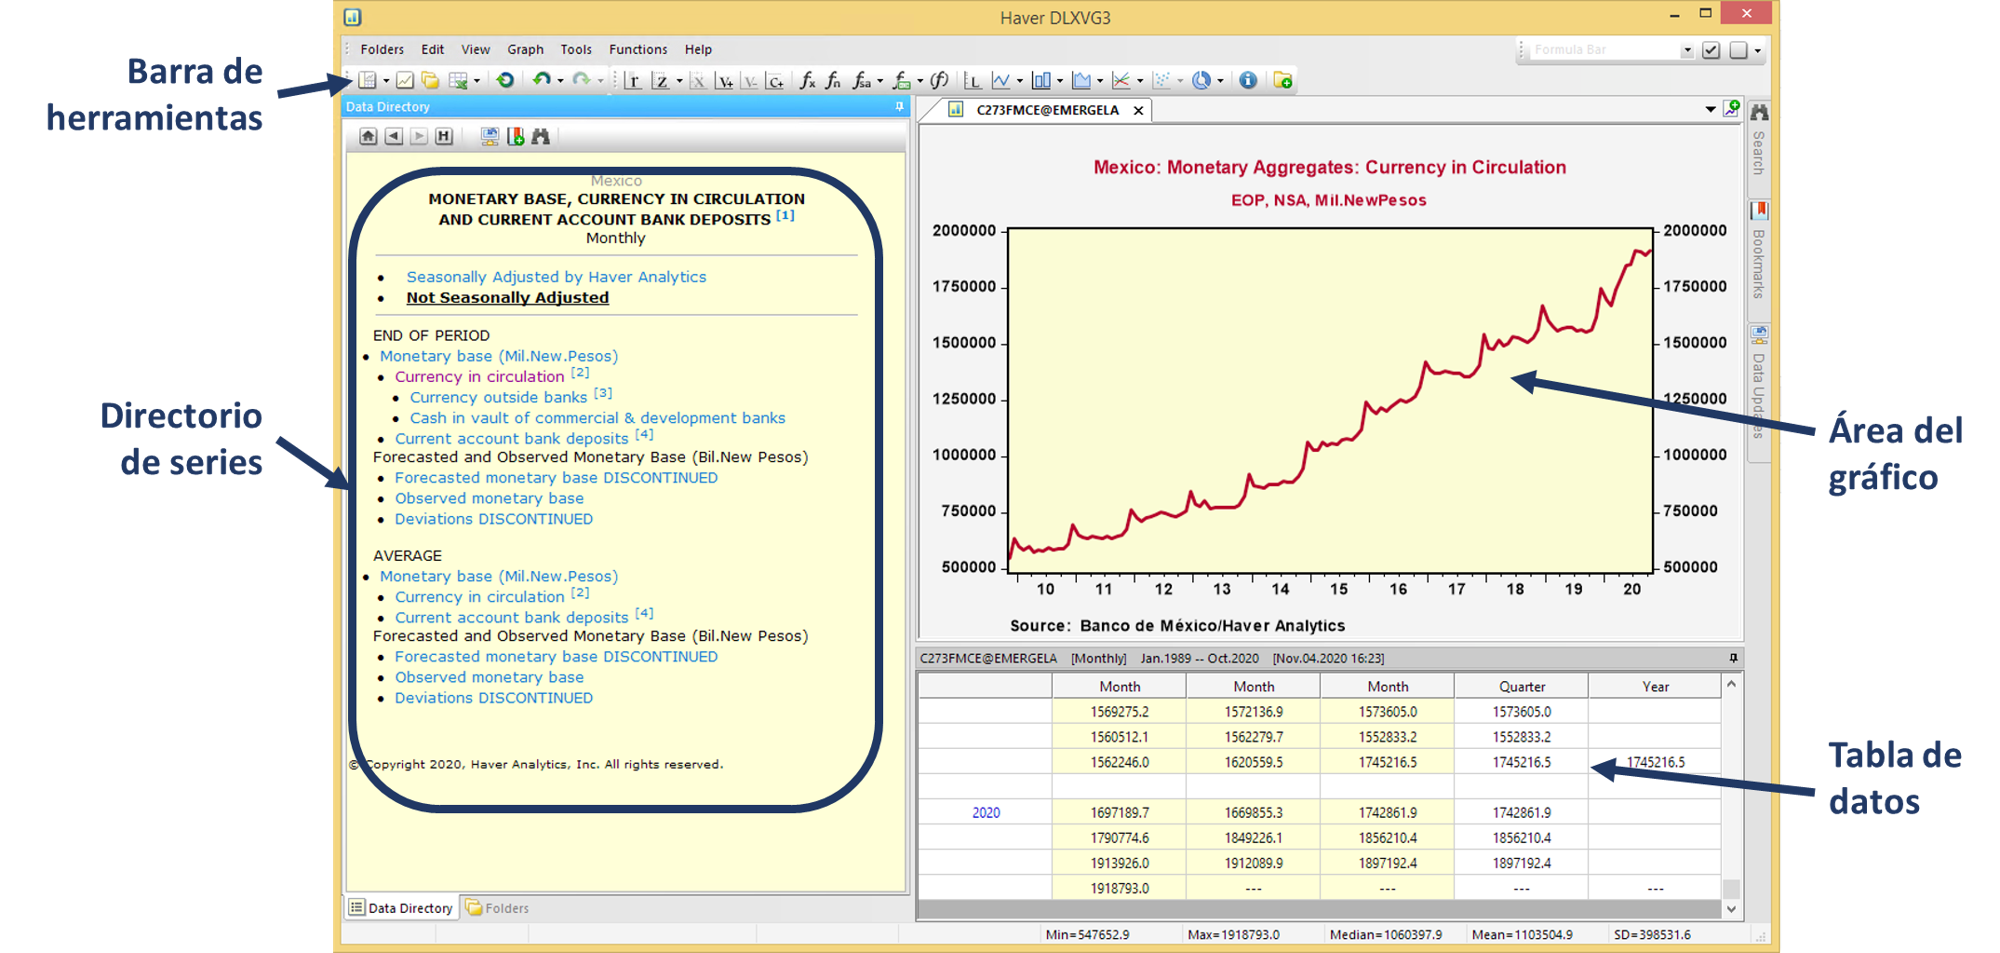
\includegraphics[width=1\linewidth]{_img/dlx_app} 

}

\caption{Aplicación DLX para Haver Analytics.}\label{fig:app}
\end{figure}

\hypertarget{add-in-para-excel}{%
\section{Add-in para Excel}\label{add-in-para-excel}}

Las series de Haver Analytics se pueden consultar directamente desde Excel utilizando el \emph{add-in} DLX. Para verificar si se tiene instalado este complemento, en Excel deberías tener una pestaña que diga \textbf{DLX}.

Una vez seleccionada la pestaña, se deben seguir los siguientes pasos:

\begin{enumerate}
\def\labelenumi{\arabic{enumi}.}
\item
  \textbf{Seleccionar las series}, dando click en el ícono \textbf{DLXVG3}, el cual abre un catálogo para seleccionar las series.
\item
  \textbf{Seleccionar rango}, usando el ícono \textbf{DLXRanger}, seleccionar la frecuencia y rangod e fechas de las series de tiempo.
\item
  \textbf{Correr la consulta}, la cual se puede correr para la hoja seleccionada dando click en ``Retrieve Worksheet'', o todas las series del archivo dando click en ``Retrieve Workbook''.
\end{enumerate}

\begin{figure}

{\centering 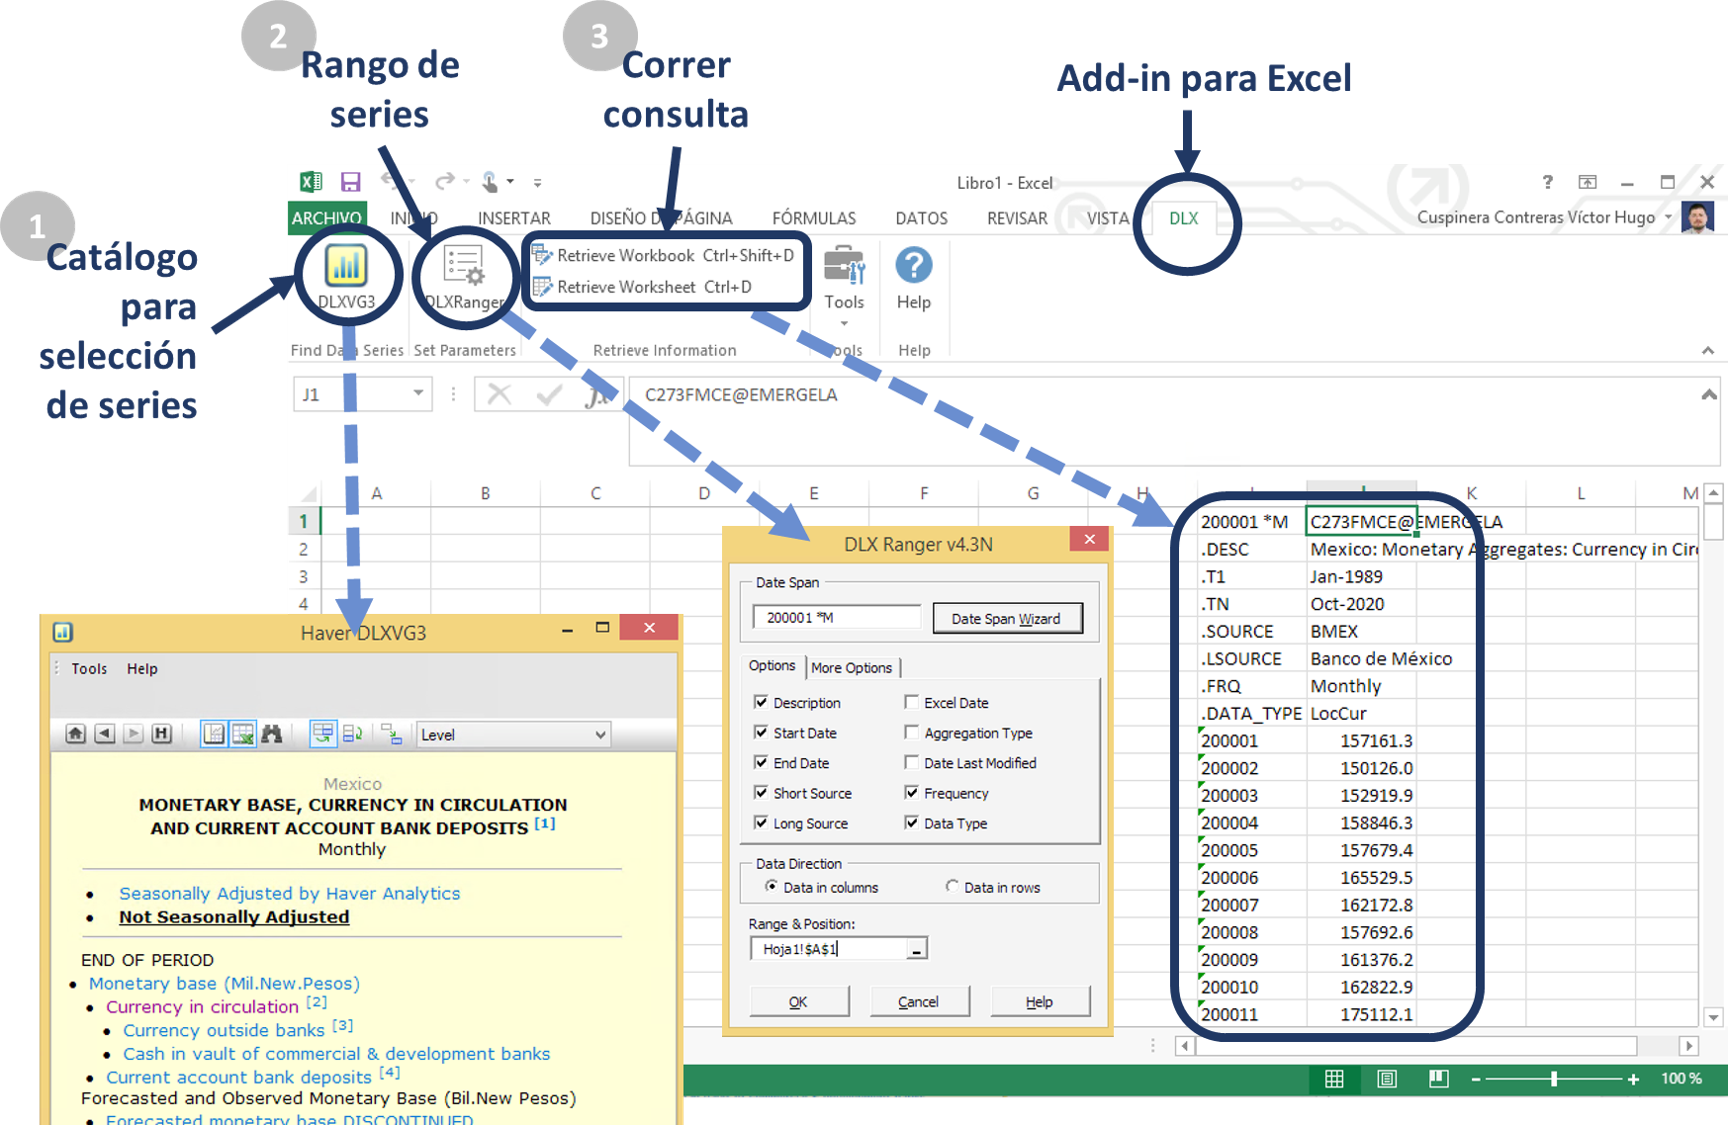
\includegraphics[width=1\linewidth]{_img/dlx_add_in} 

}

\caption{DLX add-in para Excel.}\label{fig:addin}
\end{figure}

\hypertarget{consulta-con-r}{%
\section{Consulta con R}\label{consulta-con-r}}

El primer paso es instalar el paquete, corriendo la siguiente línea desde R o RStudio:

\texttt{install.packages("Haver",\ repos="http://www.haver.com/r/")}

Después habrá que llamar las librerías y fijar la ruta a las bases de datos con los siguientes comandos:

\begin{Shaded}
\begin{Highlighting}[]
\CommentTok{# llamar librería de Haver Analytics y tidyverse}
\KeywordTok{library}\NormalTok{(Haver)}
\KeywordTok{library}\NormalTok{(tidyverse)}
\end{Highlighting}
\end{Shaded}

\begin{verbatim}
## Warning: package 'tidyverse' was built under R version 4.0.3
\end{verbatim}

\begin{Shaded}
\begin{Highlighting}[]
\CommentTok{# fijar la ruta de las bases de datos}
\KeywordTok{haver.path}\NormalTok{()}
\end{Highlighting}
\end{Shaded}

\begin{verbatim}
## [1] "\\\\bmapps\\Bases de Informacion\\DLX\\DATA\\"
\end{verbatim}

Posteriormente hay que llamar a las series que nos interesen, y su metadata, las cuales se pueden graficar o manipular.

\begin{Shaded}
\begin{Highlighting}[]
\CommentTok{# ejemplo de consulta de serie}
\NormalTok{currency <-}\StringTok{ }\KeywordTok{haver.data}\NormalTok{(}\DataTypeTok{codes=}\KeywordTok{c}\NormalTok{(}\StringTok{"c273fmce"}\NormalTok{), }\DataTypeTok{database =} \StringTok{"EMERGELA"}\NormalTok{, }\DataTypeTok{freq=}\StringTok{"q"}\NormalTok{, }\DataTypeTok{start=}\KeywordTok{as.Date}\NormalTok{(}\StringTok{"2010-01-01"}\NormalTok{, }\DataTypeTok{format=}\StringTok{"%Y-%m-%d"}\NormalTok{))}

\CommentTok{# cambio de nombre}
\KeywordTok{colnames}\NormalTok{(currency)[}\KeywordTok{colnames}\NormalTok{(currency) }\OperatorTok{==}\StringTok{ "c273fmce"}\NormalTok{] <-}\StringTok{ "Currency_in_Circulation"}

\CommentTok{# ver inicio de serie para identificar su estructura}
\NormalTok{currency }\OperatorTok\StringTok{ }\KeywordTok{head}\NormalTok{()}
\end{Highlighting}
\end{Shaded}

\begin{verbatim}
##         Currency_in_Circulation
## 2010-Q1                597193.9
## 2010-Q2                577815.5
## 2010-Q3                588091.8
## 2010-Q4                693423.1
## 2011-Q1                634711.8
## 2011-Q2                635323.3
\end{verbatim}

\begin{Shaded}
\begin{Highlighting}[]
\CommentTok{# imprimir metadata}
\KeywordTok{haver.datamd}\NormalTok{(currency)}
\end{Highlighting}
\end{Shaded}

\begin{verbatim}
## 
## HaverMetaData object:
## 
##   database code     startdate  enddate    frequency numobs
## 1 emergela c273fmce 1989-01-31 2020-10-31 M         382   
##   descriptor                    
## 1 Mexico: Monetary Aggregates:..
## 
##   # of series records : 1
##   database path       : \\bmapps\Bases de Informacion\DLX\DATA\
##   query date and time : 2020-11-30 22:53:19
\end{verbatim}

\begin{Shaded}
\begin{Highlighting}[]
\CommentTok{# convertir serie a data.frame}
\NormalTok{currency <-}\StringTok{ }\KeywordTok{data.frame}\NormalTok{(currency)}
\NormalTok{currency}\OperatorTok{$}\NormalTok{date <-}\StringTok{ }\KeywordTok{row.names}\NormalTok{(currency)}

\CommentTok{# gráficar serie}
\NormalTok{currency }\OperatorTok\StringTok{ }\KeywordTok{ggplot}\NormalTok{() }\OperatorTok{+}
\StringTok{  }\KeywordTok{geom_line}\NormalTok{(}\KeywordTok{aes}\NormalTok{(}\DataTypeTok{x =}\NormalTok{ date, }
                \DataTypeTok{y =}\NormalTok{ Currency_in_Circulation, }
                \DataTypeTok{group =} \DecValTok{1}\NormalTok{), }\DataTypeTok{color=}\StringTok{"darkred"}\NormalTok{) }\OperatorTok{+}
\StringTok{  }\KeywordTok{theme_bw}\NormalTok{() }\OperatorTok{+}
\StringTok{  }\KeywordTok{theme}\NormalTok{(}\DataTypeTok{axis.text.x =} \KeywordTok{element_text}\NormalTok{(}\DataTypeTok{angle =} \DecValTok{60}\NormalTok{, }\DataTypeTok{vjust =} \FloatTok{0.5}\NormalTok{)) }\OperatorTok{+}\StringTok{ }
\StringTok{  }\KeywordTok{scale_x_discrete}\NormalTok{(}\DataTypeTok{breaks =}\NormalTok{ currency}\OperatorTok{$}\NormalTok{date[}\KeywordTok{seq}\NormalTok{(}\DecValTok{1}\NormalTok{, }\KeywordTok{length}\NormalTok{(currency}\OperatorTok{$}\NormalTok{date), }\DataTypeTok{by =} \DecValTok{2}\NormalTok{)])}\OperatorTok{+}
\StringTok{  }\KeywordTok{scale_y_continuous}\NormalTok{(}\DataTypeTok{limits =} \KeywordTok{c}\NormalTok{(}\DecValTok{500000}\NormalTok{, }\DecValTok{2000000}\NormalTok{), }
                     \DataTypeTok{labels =}\NormalTok{ scales}\OperatorTok{::}\NormalTok{dollar) }\OperatorTok{+}
\StringTok{  }\KeywordTok{labs}\NormalTok{(}\DataTypeTok{x =} \StringTok{"Date"}\NormalTok{, }\DataTypeTok{y =} \StringTok{"Currency in Circulation"}\NormalTok{)}
\end{Highlighting}
\end{Shaded}

\begin{verbatim}
## Warning: Removed 1 row(s) containing missing values (geom_path).
\end{verbatim}

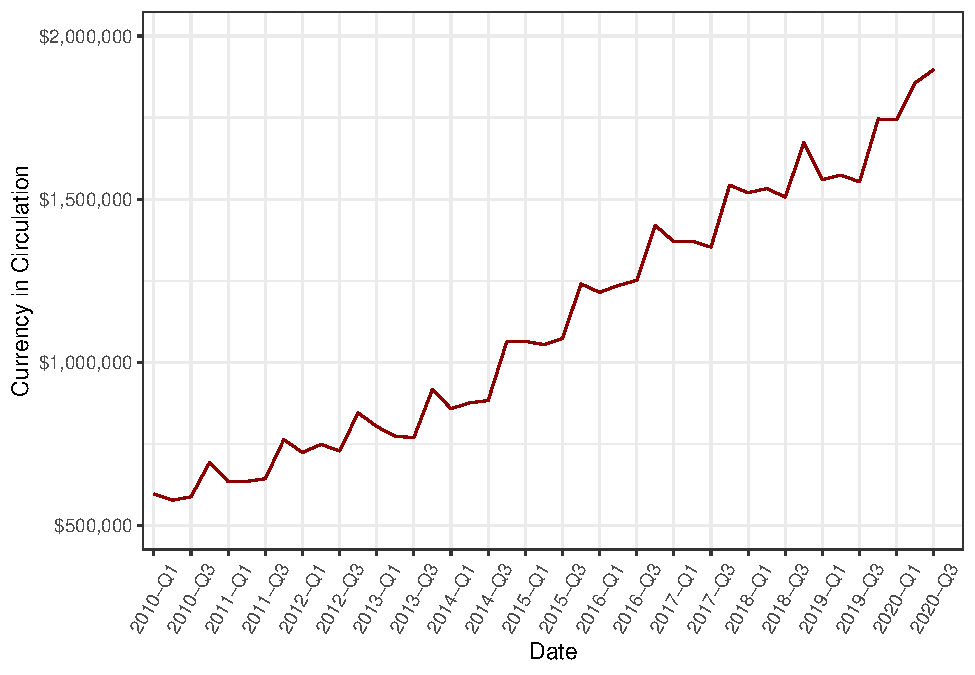
\includegraphics{Guide_Haver_Analytics_files/figure-latex/consulta_en_R-1.pdf}

Para acceder a la guía completa del paquete \texttt{Haver} en R puedes:

\begin{itemize}
\item
  correr el siguiente comando en RStudio: \texttt{help("Haver")}, o
\item
  ingresar a la página oficial de \href{http://www.haver.com}{Haver Analytics}, dar click en \emph{Client area} donde te pedirán un código de usuario el cual te lo pueden dar a través del correo \href{mailto:data@haver.com}{\nolinkurl{data@haver.com}}, seleccionar \emph{Resources}, después ingresar en \emph{Using DLX Data with Third Party Statistical Software}, y selecionar la \textbf{guía de usuario para R} \citep{haver_r}.
\end{itemize}

\hypertarget{consulta-con-python}{%
\section{Consulta con Python}\label{consulta-con-python}}

El primer paso es instalar el paquete de Haver en Python, lo cual se puede relaizar de la siguiente manera:\footnote{Basado en script para uso de Haver por primera vez, compartido por \citet{haver_python_install} de Haver Analytics.}

\begin{itemize}
\tightlist
\item
  \textbf{interfaz}: desde PowerShell/Terminal, correr el siguiente comando:
\end{itemize}

\begin{verbatim}
pip install Haver --extra-index-url https://urldefense.proofpoint.com/v2/url?u=http-3A__www.haver.com_Python&d=DwIGAg&c=AKs6EwELrBZKOG9H-C2eL9nCFyT6KLG5z2zMuwOnNTA&r=1xye9t3tMb09G6CmueM5cDX4CvWN9LC-lHqLRumN6Ls&m=OzpuOY3Klwky0-MpBXHqoFFIN7cUKTHg3FHaKc18LaY&s=yWr_0mX3wkhn60y5OE2ZDv2Hb-rIrBaVzLVAmE0ghkA&e=  --trusted-host https://urldefense.proofpoint.com/v2/url?u=http-3A__www.haver.com&d=DwIGAg&c=AKs6EwELrBZKOG9H-C2eL9nCFyT6KLG5z2zMuwOnNTA&r=1xye9t3tMb09G6CmueM5cDX4CvWN9LC-lHqLRumN6Ls&m=OzpuOY3Klwky0-MpBXHqoFFIN7cUKTHg3FHaKc18LaY&s=KJOUUR_knntVVk2lyRqTBi8i7JLK_cfqqjh5Kcu1ReE&e=
\end{verbatim}

\ldots si esto no funciona, se tiene que realizar una instalación manual.

\begin{itemize}
\tightlist
\item
  \textbf{manual}:

  \begin{enumerate}
  \def\labelenumi{\arabic{enumi}.}
  \tightlist
  \item
    ingresar a la página \url{http://www.haver.com/Python/Haver/},
  \item
    descargar el archivo de formato \texttt{wheel}, con extensión `whl', que corresponda a la versión que tengas instalada de Python. Por ejemplo, el archivo \texttt{Haver-1.1.0-cp35-cp35mwin\_amd64.whl} corresponde a la versión instalada de Python 3.5
  \item
    Desde PowerShell/Terminal, ir a la carpeta donde se encuentre el archivo descargado en el punto anterior y correr el siguiente comando reemplazando `archivo\_wheel' por el nombre del archivo descargado
  \end{enumerate}
\end{itemize}

\begin{verbatim}
pip install archivo_wheel.whl
\end{verbatim}

Ya instalado el paquete de Haver en Python, podemos empezar a trabajar ya sea directamente con Python o a través de alguna de sus interfaces (Jupyter Lab, Jupyter Notebook, Spider). Lo primero que tenemos que hacer es llamar las librerías y fijar la ruta a las bases de datos con los siguientes comandos:

\begin{Shaded}
\begin{Highlighting}[]
\CommentTok{# llamar librerias de Python}
\ImportTok{import}\NormalTok{ Haver }\ImportTok{as}\NormalTok{ hv}
\ImportTok{import}\NormalTok{ pandas }\ImportTok{as}\NormalTok{ pd}
\ImportTok{import}\NormalTok{ numpy }\ImportTok{as}\NormalTok{ np}
\ImportTok{import}\NormalTok{ altair }\ImportTok{as}\NormalTok{ alt}

\CommentTok{# fijar la ruta de haver}
\NormalTok{hv.path()}
\end{Highlighting}
\end{Shaded}

\begin{verbatim}
## '\\\\bmapps\\Bases de Informacion\\dlx\\data\\'
\end{verbatim}

Posteriormente hay que llamar a las series que nos interesen, y su metadata, las cuales se pueden graficar o manipular.

\begin{verbatim}
# ejemplo de consulta de serie
currency = hv.data(codes=["c273fmce"], database="EMERGELA", 
                   frequency="q", startdate="2010-01-01")

# cambio de nombre
currency = currency.reset_index().dropna().rename(columns = {"index": "fecha", "c273fmce":"Currency_in_Circulation"})
currency.fecha = [str(i) for i in currency.fecha]

# obtener metadata
currency_md = hv.metadata(codes=["c273fmce"], database="EMERGELA").T

# graficar
alt.Chart(currency).mark_line(color="darkred").encode(
    x=alt.X('fecha', title="Date"),
    y=alt.Y('Currency_in_Circulation:Q', title="Currency in Circulation"),
    tooltip=['fecha', 'Currency_in_Circulation']
).properties(
    width=500
)
\end{verbatim}

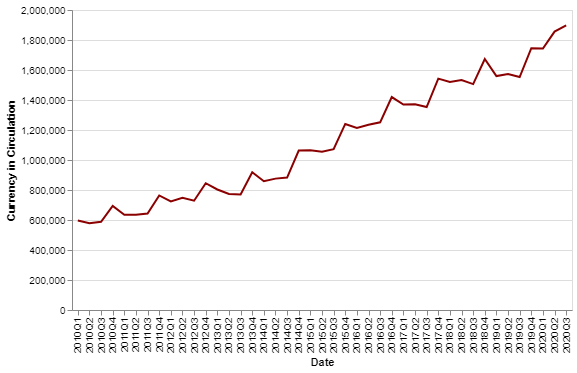
\includegraphics{_img/python_plot.png}

Para acceder a la guía completa del paquete \texttt{Haver} en Python puedes:

\begin{itemize}
\tightlist
\item
  ingresar a la página oficial de \href{http://www.haver.com}{Haver Analytics}, dar click en \emph{Client area} donde te pedirán un código de usuario el cual te lo pueden dar a través del correo \href{mailto:data@haver.com}{\nolinkurl{data@haver.com}}, seleccionar \emph{Resources}, después ingresar en \emph{Using DLX Data with Third Party Statistical Software}, y selecionar la \textbf{guía de usuario para Python} \citep{haver_python}.
\end{itemize}

\hypertarget{series}{%
\chapter{Series}\label{series}}

Como se mencionó en la introducción, el Banco tiene contratado una subscripción a algunas de las bases de datos de esta empresa, las cuales contienen diversas series.

\href{http://webinterno/centro-de-informacion-electronica/acceso-a-recursos-electronicos/bases-de-datos-con-informacion-estadistica/haver-analytics-global/haver-analytics-global--.html}{En este link} podrás para revisar las bases de datos contratadas por Banxico a Haver Analytics.

Es importante mencionar que aunque algunas serie se encuentran replicadas en bases de datos distintas, estas pueden tener algunas pequeñas modificaciones para ajustarse a la periodicidad o formato de las otras series de la base de datos.

\hypertarget{bases-de-datos}{%
\section{Bases de datos}\label{bases-de-datos}}

En el siguiente cuadro se muestran las 29 bases de datos contratadas por Banxico, junto con su descripción y número de series.\footnote{Información consultada el 2020-11-24 en DLX y a través de Python.}

\begin{longtable}[]{@{}lllr@{}}
\toprule
\begin{minipage}[b]{0.20\columnwidth}\raggedright
Database\strut
\end{minipage} & \begin{minipage}[b]{0.12\columnwidth}\raggedright
Group\strut
\end{minipage} & \begin{minipage}[b]{0.26\columnwidth}\raggedright
Description\strut
\end{minipage} & \begin{minipage}[b]{0.30\columnwidth}\raggedleft
No.~de series\strut
\end{minipage}\tabularnewline
\midrule
\endhead
\begin{minipage}[t]{0.20\columnwidth}\raggedright
USECON\strut
\end{minipage} & \begin{minipage}[t]{0.12\columnwidth}\raggedright
U.S. Detail\strut
\end{minipage} & \begin{minipage}[t]{0.26\columnwidth}\raggedright
United States Economic Statistics\strut
\end{minipage} & \begin{minipage}[t]{0.30\columnwidth}\raggedleft
63,934\strut
\end{minipage}\tabularnewline
\begin{minipage}[t]{0.20\columnwidth}\raggedright
SURVEYS\strut
\end{minipage} & \begin{minipage}[t]{0.12\columnwidth}\raggedright
U.S. Detail\strut
\end{minipage} & \begin{minipage}[t]{0.26\columnwidth}\raggedright
Surveys Including FED Special Series\strut
\end{minipage} & \begin{minipage}[t]{0.30\columnwidth}\raggedleft
68,888\strut
\end{minipage}\tabularnewline
\begin{minipage}[t]{0.20\columnwidth}\raggedright
SURVEYW\strut
\end{minipage} & \begin{minipage}[t]{0.12\columnwidth}\raggedright
U.S. Detail\strut
\end{minipage} & \begin{minipage}[t]{0.26\columnwidth}\raggedright
Weekly Surveys of Economic Activity\strut
\end{minipage} & \begin{minipage}[t]{0.30\columnwidth}\raggedleft
32,164\strut
\end{minipage}\tabularnewline
\begin{minipage}[t]{0.20\columnwidth}\raggedright
\strut
\end{minipage} & \begin{minipage}[t]{0.12\columnwidth}\raggedright
\strut
\end{minipage} & \begin{minipage}[t]{0.26\columnwidth}\raggedright
\strut
\end{minipage} & \begin{minipage}[t]{0.30\columnwidth}\raggedleft
\strut
\end{minipage}\tabularnewline
\begin{minipage}[t]{0.20\columnwidth}\raggedright
GLSECTOR\strut
\end{minipage} & \begin{minipage}[t]{0.12\columnwidth}\raggedright
Industry Detail\strut
\end{minipage} & \begin{minipage}[t]{0.26\columnwidth}\raggedright
Global Sector Statistics\strut
\end{minipage} & \begin{minipage}[t]{0.30\columnwidth}\raggedleft
277,412\strut
\end{minipage}\tabularnewline
\begin{minipage}[t]{0.20\columnwidth}\raggedright
\strut
\end{minipage} & \begin{minipage}[t]{0.12\columnwidth}\raggedright
\strut
\end{minipage} & \begin{minipage}[t]{0.26\columnwidth}\raggedright
\strut
\end{minipage} & \begin{minipage}[t]{0.30\columnwidth}\raggedleft
\strut
\end{minipage}\tabularnewline
\begin{minipage}[t]{0.20\columnwidth}\raggedright
WARDSINT\strut
\end{minipage} & \begin{minipage}[t]{0.12\columnwidth}\raggedright
Automotive Detail\strut
\end{minipage} & \begin{minipage}[t]{0.26\columnwidth}\raggedright
Global, Ward's Automotive Data\strut
\end{minipage} & \begin{minipage}[t]{0.30\columnwidth}\raggedleft
528\strut
\end{minipage}\tabularnewline
\begin{minipage}[t]{0.20\columnwidth}\raggedright
\strut
\end{minipage} & \begin{minipage}[t]{0.12\columnwidth}\raggedright
\strut
\end{minipage} & \begin{minipage}[t]{0.26\columnwidth}\raggedright
\strut
\end{minipage} & \begin{minipage}[t]{0.30\columnwidth}\raggedleft
\strut
\end{minipage}\tabularnewline
\begin{minipage}[t]{0.20\columnwidth}\raggedright
G10\strut
\end{minipage} & \begin{minipage}[t]{0.12\columnwidth}\raggedright
Advance Ecopnomies\strut
\end{minipage} & \begin{minipage}[t]{0.26\columnwidth}\raggedright
Country Summary Statistics\strut
\end{minipage} & \begin{minipage}[t]{0.30\columnwidth}\raggedleft
17,968\strut
\end{minipage}\tabularnewline
\begin{minipage}[t]{0.20\columnwidth}\raggedright
\strut
\end{minipage} & \begin{minipage}[t]{0.12\columnwidth}\raggedright
\strut
\end{minipage} & \begin{minipage}[t]{0.26\columnwidth}\raggedright
\strut
\end{minipage} & \begin{minipage}[t]{0.30\columnwidth}\raggedleft
\strut
\end{minipage}\tabularnewline
\begin{minipage}[t]{0.20\columnwidth}\raggedright
EMERGE\strut
\end{minipage} & \begin{minipage}[t]{0.12\columnwidth}\raggedright
Emerging Markets\strut
\end{minipage} & \begin{minipage}[t]{0.26\columnwidth}\raggedright
Country Summary Statistics\strut
\end{minipage} & \begin{minipage}[t]{0.30\columnwidth}\raggedleft
42,103\strut
\end{minipage}\tabularnewline
\begin{minipage}[t]{0.20\columnwidth}\raggedright
EMERGELA\strut
\end{minipage} & \begin{minipage}[t]{0.12\columnwidth}\raggedright
Emerging Markets\strut
\end{minipage} & \begin{minipage}[t]{0.26\columnwidth}\raggedright
Latin America\strut
\end{minipage} & \begin{minipage}[t]{0.30\columnwidth}\raggedleft
70,705\strut
\end{minipage}\tabularnewline
\begin{minipage}[t]{0.20\columnwidth}\raggedright
EMERGEPR\strut
\end{minipage} & \begin{minipage}[t]{0.12\columnwidth}\raggedright
Emerging Markets\strut
\end{minipage} & \begin{minipage}[t]{0.26\columnwidth}\raggedright
Asia Pacific\strut
\end{minipage} & \begin{minipage}[t]{0.30\columnwidth}\raggedleft
256,779\strut
\end{minipage}\tabularnewline
\begin{minipage}[t]{0.20\columnwidth}\raggedright
EMERGECW\strut
\end{minipage} & \begin{minipage}[t]{0.12\columnwidth}\raggedright
Emerging Markets\strut
\end{minipage} & \begin{minipage}[t]{0.26\columnwidth}\raggedright
Central, Eastern Europe \& Western Asia\strut
\end{minipage} & \begin{minipage}[t]{0.30\columnwidth}\raggedleft
252,574\strut
\end{minipage}\tabularnewline
\begin{minipage}[t]{0.20\columnwidth}\raggedright
EMERGEMA\strut
\end{minipage} & \begin{minipage}[t]{0.12\columnwidth}\raggedright
Emerging Markets\strut
\end{minipage} & \begin{minipage}[t]{0.26\columnwidth}\raggedright
Middle East \& Africa\strut
\end{minipage} & \begin{minipage}[t]{0.30\columnwidth}\raggedleft
152,190\strut
\end{minipage}\tabularnewline
\begin{minipage}[t]{0.20\columnwidth}\raggedright
CHINA\strut
\end{minipage} & \begin{minipage}[t]{0.12\columnwidth}\raggedright
Emerging Markets\strut
\end{minipage} & \begin{minipage}[t]{0.26\columnwidth}\raggedright
CEIC Premium China Database\strut
\end{minipage} & \begin{minipage}[t]{0.30\columnwidth}\raggedleft
377,004\strut
\end{minipage}\tabularnewline
\begin{minipage}[t]{0.20\columnwidth}\raggedright
\strut
\end{minipage} & \begin{minipage}[t]{0.12\columnwidth}\raggedright
\strut
\end{minipage} & \begin{minipage}[t]{0.26\columnwidth}\raggedright
\strut
\end{minipage} & \begin{minipage}[t]{0.30\columnwidth}\raggedleft
\strut
\end{minipage}\tabularnewline
\begin{minipage}[t]{0.20\columnwidth}\raggedright
EIUIAMER\strut
\end{minipage} & \begin{minipage}[t]{0.12\columnwidth}\raggedright
EIU Market Indicators\strut
\end{minipage} & \begin{minipage}[t]{0.26\columnwidth}\raggedright
Americas\strut
\end{minipage} & \begin{minipage}[t]{0.30\columnwidth}\raggedleft
4,948\strut
\end{minipage}\tabularnewline
\begin{minipage}[t]{0.20\columnwidth}\raggedright
EIUIASIA\strut
\end{minipage} & \begin{minipage}[t]{0.12\columnwidth}\raggedright
EIU Market Indicators\strut
\end{minipage} & \begin{minipage}[t]{0.26\columnwidth}\raggedright
Asia \& Australasia\strut
\end{minipage} & \begin{minipage}[t]{0.30\columnwidth}\raggedleft
6,957\strut
\end{minipage}\tabularnewline
\begin{minipage}[t]{0.20\columnwidth}\raggedright
EIUIEEUR\strut
\end{minipage} & \begin{minipage}[t]{0.12\columnwidth}\raggedright
EIU Market Indicators\strut
\end{minipage} & \begin{minipage}[t]{0.26\columnwidth}\raggedright
Eastern Europe\strut
\end{minipage} & \begin{minipage}[t]{0.30\columnwidth}\raggedleft
4,406\strut
\end{minipage}\tabularnewline
\begin{minipage}[t]{0.20\columnwidth}\raggedright
EIUIWEUR\strut
\end{minipage} & \begin{minipage}[t]{0.12\columnwidth}\raggedright
EIU Market Indicators\strut
\end{minipage} & \begin{minipage}[t]{0.26\columnwidth}\raggedright
Western Europe\strut
\end{minipage} & \begin{minipage}[t]{0.30\columnwidth}\raggedleft
7,543\strut
\end{minipage}\tabularnewline
\begin{minipage}[t]{0.20\columnwidth}\raggedright
EIUIMENA\strut
\end{minipage} & \begin{minipage}[t]{0.12\columnwidth}\raggedright
EIU Market Indicators\strut
\end{minipage} & \begin{minipage}[t]{0.26\columnwidth}\raggedright
Middle East \& North Africa\strut
\end{minipage} & \begin{minipage}[t]{0.30\columnwidth}\raggedleft
2,534\strut
\end{minipage}\tabularnewline
\begin{minipage}[t]{0.20\columnwidth}\raggedright
EIUISUBS\strut
\end{minipage} & \begin{minipage}[t]{0.12\columnwidth}\raggedright
EIU Market Indicators\strut
\end{minipage} & \begin{minipage}[t]{0.26\columnwidth}\raggedright
Sub-Saharan Africa\strut
\end{minipage} & \begin{minipage}[t]{0.30\columnwidth}\raggedleft
1,,381\strut
\end{minipage}\tabularnewline
\begin{minipage}[t]{0.20\columnwidth}\raggedright
EIUIREGS\strut
\end{minipage} & \begin{minipage}[t]{0.12\columnwidth}\raggedright
EIU Market Indicators\strut
\end{minipage} & \begin{minipage}[t]{0.26\columnwidth}\raggedright
World \& Regional Aggregates\strut
\end{minipage} & \begin{minipage}[t]{0.30\columnwidth}\raggedleft
4,170\strut
\end{minipage}\tabularnewline
\begin{minipage}[t]{0.20\columnwidth}\raggedright
\strut
\end{minipage} & \begin{minipage}[t]{0.12\columnwidth}\raggedright
\strut
\end{minipage} & \begin{minipage}[t]{0.26\columnwidth}\raggedright
\strut
\end{minipage} & \begin{minipage}[t]{0.30\columnwidth}\raggedleft
\strut
\end{minipage}\tabularnewline
\begin{minipage}[t]{0.20\columnwidth}\raggedright
IIFDATA\strut
\end{minipage} & \begin{minipage}[t]{0.12\columnwidth}\raggedright
Institute of International Finance Forecasts\strut
\end{minipage} & \begin{minipage}[t]{0.26\columnwidth}\raggedright
IIF Forecasts\strut
\end{minipage} & \begin{minipage}[t]{0.30\columnwidth}\raggedleft
16,161\strut
\end{minipage}\tabularnewline
\begin{minipage}[t]{0.20\columnwidth}\raggedright
\strut
\end{minipage} & \begin{minipage}[t]{0.12\columnwidth}\raggedright
\strut
\end{minipage} & \begin{minipage}[t]{0.26\columnwidth}\raggedright
\strut
\end{minipage} & \begin{minipage}[t]{0.30\columnwidth}\raggedleft
\strut
\end{minipage}\tabularnewline
\begin{minipage}[t]{0.20\columnwidth}\raggedright
FELATA\strut
\end{minipage} & \begin{minipage}[t]{0.12\columnwidth}\raggedright
Focuseconomics Consensus Forecasts\strut
\end{minipage} & \begin{minipage}[t]{0.26\columnwidth}\raggedright
Latin \& Central America\strut
\end{minipage} & \begin{minipage}[t]{0.30\columnwidth}\raggedleft
7,703\strut
\end{minipage}\tabularnewline
\begin{minipage}[t]{0.20\columnwidth}\raggedright
FEAANZ\strut
\end{minipage} & \begin{minipage}[t]{0.12\columnwidth}\raggedright
Focuseconomics Consensus Forecasts\strut
\end{minipage} & \begin{minipage}[t]{0.26\columnwidth}\raggedright
Asia \& Australia/New Zealand\strut
\end{minipage} & \begin{minipage}[t]{0.30\columnwidth}\raggedleft
8,069\strut
\end{minipage}\tabularnewline
\begin{minipage}[t]{0.20\columnwidth}\raggedright
FEMAJR\strut
\end{minipage} & \begin{minipage}[t]{0.12\columnwidth}\raggedright
Focuseconomics Consensus Forecasts\strut
\end{minipage} & \begin{minipage}[t]{0.26\columnwidth}\raggedright
Major Economies \& Euro Area\strut
\end{minipage} & \begin{minipage}[t]{0.30\columnwidth}\raggedleft
13,114\strut
\end{minipage}\tabularnewline
\begin{minipage}[t]{0.20\columnwidth}\raggedright
FEEEUR\strut
\end{minipage} & \begin{minipage}[t]{0.12\columnwidth}\raggedright
Focuseconomics Consensus Forecasts\strut
\end{minipage} & \begin{minipage}[t]{0.26\columnwidth}\raggedright
Eastern Europe\strut
\end{minipage} & \begin{minipage}[t]{0.30\columnwidth}\raggedleft
8,465\strut
\end{minipage}\tabularnewline
\begin{minipage}[t]{0.20\columnwidth}\raggedright
FELATAH\strut
\end{minipage} & \begin{minipage}[t]{0.12\columnwidth}\raggedright
Focuseconomics Consensus Forecasts\strut
\end{minipage} & \begin{minipage}[t]{0.26\columnwidth}\raggedright
Latin \& Central America: Historical\strut
\end{minipage} & \begin{minipage}[t]{0.30\columnwidth}\raggedleft
39,000\strut
\end{minipage}\tabularnewline
\begin{minipage}[t]{0.20\columnwidth}\raggedright
FEAANZH\strut
\end{minipage} & \begin{minipage}[t]{0.12\columnwidth}\raggedright
Focuseconomics Consensus Forecasts\strut
\end{minipage} & \begin{minipage}[t]{0.26\columnwidth}\raggedright
Asia \& Australia/New Zealand: Historical\strut
\end{minipage} & \begin{minipage}[t]{0.30\columnwidth}\raggedleft
45,970\strut
\end{minipage}\tabularnewline
\begin{minipage}[t]{0.20\columnwidth}\raggedright
FEMAJRH\strut
\end{minipage} & \begin{minipage}[t]{0.12\columnwidth}\raggedright
Focuseconomics Consensus Forecasts\strut
\end{minipage} & \begin{minipage}[t]{0.26\columnwidth}\raggedright
Major Economies \& Euro Area: Historical\strut
\end{minipage} & \begin{minipage}[t]{0.30\columnwidth}\raggedleft
67,304\strut
\end{minipage}\tabularnewline
\begin{minipage}[t]{0.20\columnwidth}\raggedright
FEEEURH\strut
\end{minipage} & \begin{minipage}[t]{0.12\columnwidth}\raggedright
Focuseconomics Consensus Forecasts\strut
\end{minipage} & \begin{minipage}[t]{0.26\columnwidth}\raggedright
Eastern Europe: Historical\strut
\end{minipage} & \begin{minipage}[t]{0.30\columnwidth}\raggedleft
48,610\strut
\end{minipage}\tabularnewline
\begin{minipage}[t]{0.20\columnwidth}\raggedright
FXRATES\strut
\end{minipage} & \begin{minipage}[t]{0.12\columnwidth}\raggedright
Focuseconomics Consensus Forecasts\strut
\end{minipage} & \begin{minipage}[t]{0.26\columnwidth}\raggedright
Currency Conversion Database\strut
\end{minipage} & \begin{minipage}[t]{0.30\columnwidth}\raggedleft
391\strut
\end{minipage}\tabularnewline
\bottomrule
\end{longtable}

\hypertarget{cuxf3digo-de-series}{%
\section{Código de Series}\label{cuxf3digo-de-series}}

Las \textbf{series} disponibles se pueden consultar de la siguiente forma:

\begin{itemize}
\tightlist
\item
  Navegando en el \emph{Directorio de Series} directamente en la aplicación DLX o en el add-in de Haver para Excel.
\item
  Consultar las series de una base de datos en particular a través de Python:
\end{itemize}

\begin{verbatim}
import Haver
Haver.metadata(database='database_code')
\end{verbatim}

El código completo de una serie se divide en 4 partes. Por ejemplo, el nombre completo de la serie de Dinero en Circulación es \texttt{C273FMCE@EMERGELA}, y se divide de la siguiente forma:

\begin{longtable}[]{@{}llll@{}}
\toprule
C & 273 & FMCE & @EMERGELA\tabularnewline
\midrule
\endhead
tipo de ajuste & país & tema de la serie & base de datos\tabularnewline
\bottomrule
\end{longtable}

Algunas series que nos podrían ser de utilidad:

\begin{longtable}[]{@{}lll@{}}
\toprule
\begin{minipage}[b]{0.20\columnwidth}\raggedright
Serie\strut
\end{minipage} & \begin{minipage}[b]{0.30\columnwidth}\raggedright
Database\strut
\end{minipage} & \begin{minipage}[b]{0.41\columnwidth}\raggedright
Descripción (en Inglés)\strut
\end{minipage}\tabularnewline
\midrule
\endhead
\begin{minipage}[t]{0.20\columnwidth}\raggedright
C273FMCE\strut
\end{minipage} & \begin{minipage}[t]{0.30\columnwidth}\raggedright
EMERGELA\strut
\end{minipage} & \begin{minipage}[t]{0.41\columnwidth}\raggedright
Mexico: Monetary Aggregates: Currency in Circulation (EOP, NSA, Mil.NewPesos)\strut
\end{minipage}\tabularnewline
\begin{minipage}[t]{0.20\columnwidth}\raggedright
C273XLDE\strut
\end{minipage} & \begin{minipage}[t]{0.30\columnwidth}\raggedright
EMERGELA\strut
\end{minipage} & \begin{minipage}[t]{0.41\columnwidth}\raggedright
Mexico: Exchange Rate (EOP, NewPeso/US\$)\strut
\end{minipage}\tabularnewline
\begin{minipage}[t]{0.20\columnwidth}\raggedright
N273XEUE\strut
\end{minipage} & \begin{minipage}[t]{0.30\columnwidth}\raggedright
EMERGELA\strut
\end{minipage} & \begin{minipage}[t]{0.41\columnwidth}\raggedright
Mexico: BoM Euro Exchange Rate (EOP, Peso/Euro)\strut
\end{minipage}\tabularnewline
\begin{minipage}[t]{0.20\columnwidth}\raggedright
N273XUKE\strut
\end{minipage} & \begin{minipage}[t]{0.30\columnwidth}\raggedright
EMERGELA\strut
\end{minipage} & \begin{minipage}[t]{0.41\columnwidth}\raggedright
Mexico: BoM UK Pound Sterling Exchange Rate (EOP, Peso/GBP)\strut
\end{minipage}\tabularnewline
\begin{minipage}[t]{0.20\columnwidth}\raggedright
N273NGDP\strut
\end{minipage} & \begin{minipage}[t]{0.30\columnwidth}\raggedright
EMERGELA\strut
\end{minipage} & \begin{minipage}[t]{0.41\columnwidth}\raggedright
Mexico: Gross Domestic Product at Market Prices (NSAAR, Mil.NewPesos)\strut
\end{minipage}\tabularnewline
\begin{minipage}[t]{0.20\columnwidth}\raggedright
N273NGPC\strut
\end{minipage} & \begin{minipage}[t]{0.30\columnwidth}\raggedright
EMERGELA\strut
\end{minipage} & \begin{minipage}[t]{0.41\columnwidth}\raggedright
Mexico: Gross Domestic Product at Market Prices (NSAAR, Mil.2013.NewPesos)\strut
\end{minipage}\tabularnewline
\begin{minipage}[t]{0.20\columnwidth}\raggedright
N273PJ\strut
\end{minipage} & \begin{minipage}[t]{0.30\columnwidth}\raggedright
EMERGELA\strut
\end{minipage} & \begin{minipage}[t]{0.41\columnwidth}\raggedright
Mexico: Consumer Price Index (NSA, Jul 16-31 2018=100)\strut
\end{minipage}\tabularnewline
\begin{minipage}[t]{0.20\columnwidth}\raggedright
N273EWUN\strut
\end{minipage} & \begin{minipage}[t]{0.30\columnwidth}\raggedright
EMERGELA\strut
\end{minipage} & \begin{minipage}[t]{0.41\columnwidth}\raggedright
Mexico: Minimum Wage: National (NSA, MXP/Day)\strut
\end{minipage}\tabularnewline
\begin{minipage}[t]{0.20\columnwidth}\raggedright
N273POP\strut
\end{minipage} & \begin{minipage}[t]{0.30\columnwidth}\raggedright
EMERGELA\strut
\end{minipage} & \begin{minipage}[t]{0.41\columnwidth}\raggedright
Mexico: Population (Persons)\strut
\end{minipage}\tabularnewline
\begin{minipage}[t]{0.20\columnwidth}\raggedright
N273TAUS\strut
\end{minipage} & \begin{minipage}[t]{0.30\columnwidth}\raggedright
EMERGELA\strut
\end{minipage} & \begin{minipage}[t]{0.41\columnwidth}\raggedright
Mexico: Tourist Arrivals by Air from United States (NSA, Persons)\strut
\end{minipage}\tabularnewline
\begin{minipage}[t]{0.20\columnwidth}\raggedright
N273TACA\strut
\end{minipage} & \begin{minipage}[t]{0.30\columnwidth}\raggedright
EMERGELA\strut
\end{minipage} & \begin{minipage}[t]{0.41\columnwidth}\raggedright
Mexico: Tourist Arrivals by Air from Canada (NSA, Persons)\strut
\end{minipage}\tabularnewline
\begin{minipage}[t]{0.20\columnwidth}\raggedright
N111FMC\strut
\end{minipage} & \begin{minipage}[t]{0.30\columnwidth}\raggedright
G10\strut
\end{minipage} & \begin{minipage}[t]{0.41\columnwidth}\raggedright
U.S.: Money Supply: Currency (NSA, Bil.\$)\strut
\end{minipage}\tabularnewline
\begin{minipage}[t]{0.20\columnwidth}\raggedright
H111FMR\strut
\end{minipage} & \begin{minipage}[t]{0.30\columnwidth}\raggedright
G10\strut
\end{minipage} & \begin{minipage}[t]{0.41\columnwidth}\raggedright
U.S.: Monetary Base (SA, Bil.\$)\strut
\end{minipage}\tabularnewline
\begin{minipage}[t]{0.20\columnwidth}\raggedright
N023FMC\strut
\end{minipage} & \begin{minipage}[t]{0.30\columnwidth}\raggedright
G10\strut
\end{minipage} & \begin{minipage}[t]{0.41\columnwidth}\raggedright
EA 11-19: MFIs: Liab: Currency in Circulation (EOP, NSA, Bil.EUR)\strut
\end{minipage}\tabularnewline
\begin{minipage}[t]{0.20\columnwidth}\raggedright
N023FMR\strut
\end{minipage} & \begin{minipage}[t]{0.30\columnwidth}\raggedright
G10\strut
\end{minipage} & \begin{minipage}[t]{0.41\columnwidth}\raggedright
EA 11-19: Monetary Base (EOP, NSA, Bil.EUR)\strut
\end{minipage}\tabularnewline
\begin{minipage}[t]{0.20\columnwidth}\raggedright
A273NETS\strut
\end{minipage} & \begin{minipage}[t]{0.30\columnwidth}\raggedright
EIUIAMOER\strut
\end{minipage} & \begin{minipage}[t]{0.41\columnwidth}\raggedright
Mexico: Internet Users (Thous)\strut
\end{minipage}\tabularnewline
\begin{minipage}[t]{0.20\columnwidth}\raggedright
A273ATPT\strut
\end{minipage} & \begin{minipage}[t]{0.30\columnwidth}\raggedright
EIUIAMOER\strut
\end{minipage} & \begin{minipage}[t]{0.41\columnwidth}\raggedright
Mexico: Air Transport: Passengers (Thous)\strut
\end{minipage}\tabularnewline
\bottomrule
\end{longtable}

Estas son algunas de las series que podrían ser útiles para el área; existen series similares a estas para un gran número de países lo cuál hace fácil su comparación.

Se recomienda revisar las series disponibles pues hay cerca de 1.9 millones de series en las 29 bases de datos contratadas por Banxico a Haver Analytics.

  \bibliography{book.bib,packages.bib}

\end{document}
